
%% Begin slides template file
\documentclass[11pt,t,usepdftitle=false,aspectratio=169]{beamer}
%% ------------------------------------------------------------------
%% - aspectratio=43: Set paper aspect ratio to 4:3.
%% - aspectratio=169: Set paper aspect ratio to 16:9.
%% ------------------------------------------------------------------

\usetheme[]{uibk}
%% ------------------------------------------------------------------
%% - foot: Add a footer line for conference name and date.
%% - logo: Add the university logo in the footer (only if 'foot' set).
%% - bigfoot/sasquatch: Larger font size in footer.
%% - nototalslidenumber: Hide the total number of slides (only if 'foot' set)
%% - license: Add CC-BY license symbol to title slide (e.g., for conference uploads)
%%   (TODO: At the moment no other licenses are supported.)
%% - licenseall: Add CC-BY license symbol to all subsequent slides slides
%% - url: use \url{} rather than \href{} on the title page
%% - nosectiontitlepage: switches off the behaviour of inserting the
%%   titlepage every time a \section is called. This makes it possible to
%%   use more than one section + thanks page and a ToC off by default.
%%   If the 'nosectiontitlepage' is set you can create UIBK title slides
%%   using the command '\uibktitlepage{}' in your document to create
%%   one or multiple title slides.
%% ------------------------------------------------------------------

%% ------------------------------------------------------------------
%% The official corporate colors of the university are predefined and
%% can be used for e.g., highlighting something. Simply use
%% \color{uibkorange} or \begin{color}{uibkorange} ... \end{color}
%% Defined colors are:
%% - uibkblue, uibkbluel, uibkorange, uibkorangel, uibkgray, uibkgraym, uibkgrayl
%% The frametitle color can be easily adjusted e.g., to black with
%% \setbeamercolor{titlelike}{fg=black}
%% ------------------------------------------------------------------

%\setbeamercolor{verbcolor}{fg=uibkorange}
%% ------------------------------------------------------------------
%% Setting a highlight color for verbatim output such as from
%% the commands \pkg, \email, \file, \dataset 
%% ------------------------------------------------------------------

\usepackage{tikz}
\usetikzlibrary{arrows}
\tikzset{>=stealth}

\usepackage{adjustbox}
\usepackage{bm}
\usepackage{amsmath}
\usepackage{listings}
\lstset{escapechar=`}

\usepackage[norndcorners,customcolors]{hf-tikz}
\hfsetbordercolor{uibkorange}
\hfsetfillcolor{uibkorangel}

%% information for the title page ('short title' is the pdf-title that is shown in viewer's titlebar)
\title[Balancing binary values]{Defending against power analysis\\ by balancing binary values}
\subtitle{\large a compiler based approach}

\author[Alexander Schl\"ogl]{\small Alexander Schl\"ogl, supervised by Univ.-Prof. Dr. Rainer B\"ohme}
%('short author' is the pdf-metadata Author)
%% If multiple authors are required and the font size is too large you
%% can overrule the font size of author and url by calling:
%\setbeamerfont{author}{size*={10pt}{10pt},series=\mdseries}
%\setbeamerfont{url}{size*={10pt}{10pt},series=\mdseries}
%\URL{}
%\subtitle{}

\date{2019-09-11}

\headerimage{2}
%% ------------------------------------------------------------------
%% The theme offers four different header images based on the
%% corporate design of the university of innsbruck. Currently
%% 1, 2, 3 and 4 is allowed as input to \headerimage{...}. Default
%% or fallback is '1'.
%% ------------------------------------------------------------------

\usepackage{graphicx}
\graphicspath{ {fig/}}

\newcommand\blfootnote[1]{%
  \begingroup
  \renewcommand\thefootnote{}\footnote{#1}%
  \addtocounter{footnote}{-1}%
  \endgroup
}
\hyphenation{consumption}
\hyphenation{algorithm}

\newcommand{\hex}[1]{\texttt{0x#1}}

\renewcommand{\neg}[1]{\ensuremath{\overline{#1}}}
\newcommand{\bsep}{\; \| \; }
\newcommand{\borr}{\mathbin{\texttt{ORR}}}
\newcommand{\band}{\mathbin{\texttt{AND}}}
\newcommand{\bxor}{\mathbin{\texttt{XOR}}}
\newcommand{\bror}{\mathbin{\texttt{ROR}}}
\newcommand{\blsl}{\mathbin{\texttt{LSL}}}
\newcommand{\trans}[2]{\ensuremath{\texttt{transform\_#1\_#2}}}

\newcommand{\binp}[5]{\ensuremath{\%#1 &= #2 &&\bsep #3 &&\bsep #4 &&\bsep #5 &&}}
\newcommand{\btrans}[6]{\ensuremath{\%#1 &= #2 &&\bsep #3 &&\bsep #4 &&\bsep #5 && \;|\ #6}}

\newcommand{\vq}{\vphantom{q}}

\begin{document}

%% ALTERNATIVE TITLEPAGE
%% The next block is how you add a titlepage with the 'nosectiontitlepage' option, which switches off
%% the default behavior of creating a titlepage every time a \section{} is defined.
%% Then you can use \section{} as it's originally intended, including a table of contents.
% \usebackgroundtemplate{\includegraphics[width=\paperwidth,height=\paperheight]{titlebackground.pdf}}
% \begin{frame}[plain]
%     \titlepage
% \end{frame}
% \addtocounter{framenumber}{-1}
% \usebackgroundtemplate{}

%% Table of Contents, if wanted:
%% this requires the 'nosectiontitlepage' option and setting \section{}'s as you want them to appear here.
%% Subsections and subordinates are suppressed in the .sty at the moment, search
%% for \setbeamertemplate{subsection} and replace the empty {} with whatever you want.
%% Although it's probably too much for a presentation, maybe for a lecture.
%% Please note: \maketitle allows you to render a uibk-style title page wherever needed
%% in the document even if 'nosectiontitlepage' option is set (note: \maketitle will not
%% create a new section and is therefore not included in \tableofcontents (if used).
% \maketitle
% \begin{frame}
%     \vspace*{1cm plus 1fil}
%     \tableofcontents
%     \vspace*{0cm plus 1fil}
% \end{frame}


%% this sets the first PDF bookmark and triggers generation of the title page
\section{Bookmark Title}

\begin{frame}
  \frametitle{Motivation}
  \begin{figure}
    \centering
    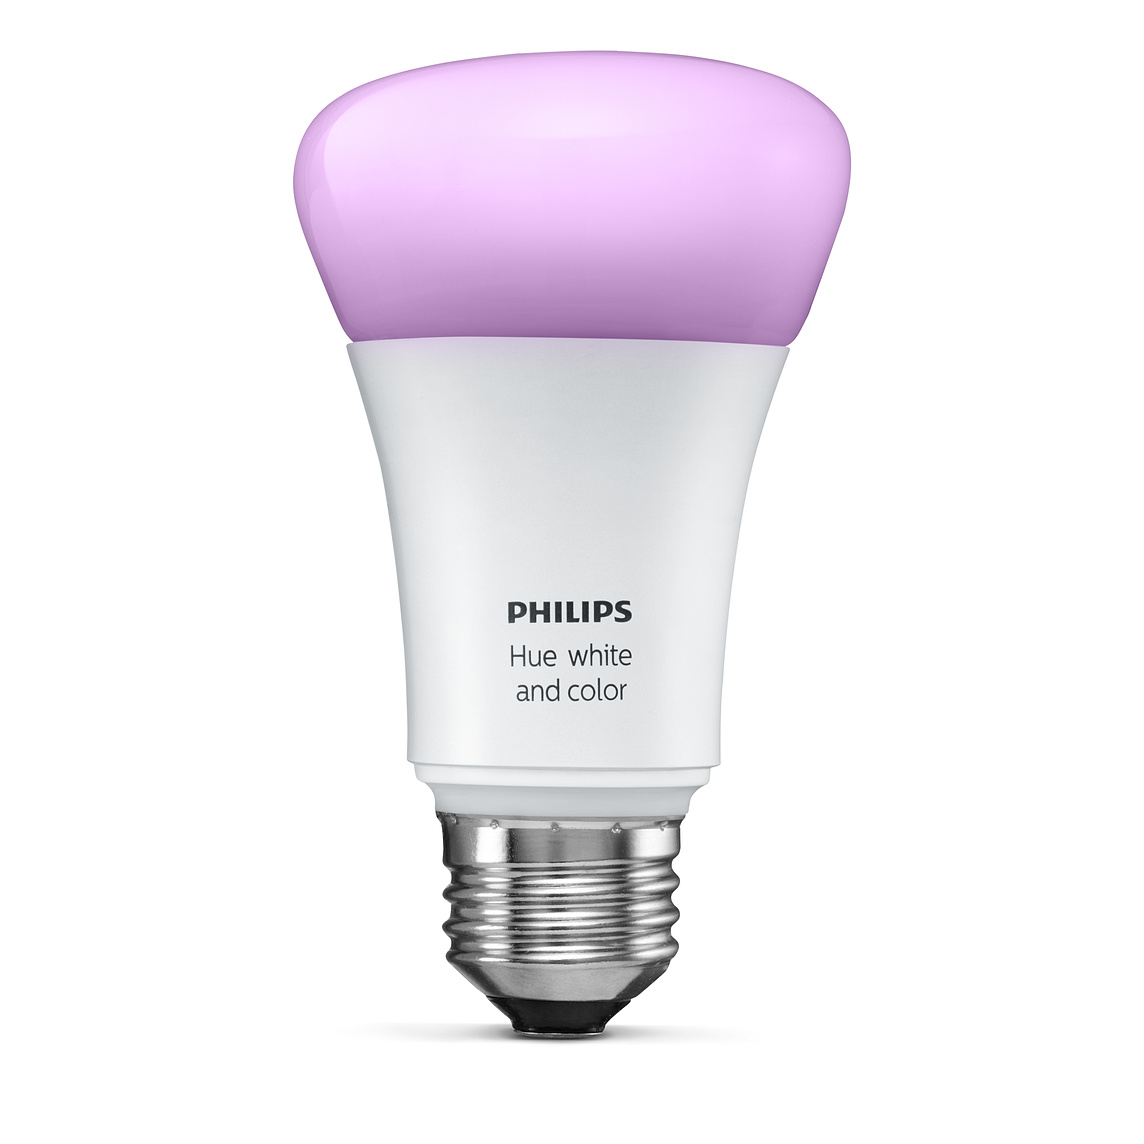
\includegraphics[width=0.4\textwidth]{hue.jpeg}
  \end{figure}
  \blfootnote{\tiny https://store.storeimages.cdn-apple.com/4982/as-images.apple.com/is/HJCC2?wid=1144\&hei=1144\&fmt=jpeg\&qlt=95\&op\_usm=0.5,0.5\&.v=0}
\end{frame}

\begin{frame}
  \frametitle{Motivation}
  \begin{figure}
    \centering
    \begin{tikzpicture}[every node/.style={draw}]
      \node (input) at (-4, 2) {\vq Input};
      \node (secret) at (-4, -2) {\vq Secret};
      \node (result) at (-0.5,0) {\vq Result};
      \node[text width=2.5cm, align=center] (power) at (4,0) {\vq Power Consumption};

      \draw[->] (input) -- (result);
      \draw[->] (secret) -- (result);
      \draw[->] (result) -- (power);

      \onslide<2>{
      \draw[->, uibkorange, line width=0.4mm] (5,-3.5) -- (-4.5, -3.5) node[midway, above, draw=none] {Power Analysis Attack};}
      \onslide<3>{
        \draw[->, uibkblue, line width=0.4mm] (5,-3.5) -- (-4.5, -3.5) node[midway, above, draw=none] {Power Analysis Attack};
        \node[uibkorange, thick] (mask) at (-4, 0) {\vq Mask};
        \draw[uibkorange, thick, ->] (mask) -- (result);

        \draw[uibkorange, line width=0.4mm] (1.45,0.15) -- (1.15,-0.15);
        \draw[uibkorange, line width=0.4mm] (1.15,0.15) -- (1.45,-0.15);

        \draw[uibkorange, thick,<-] (1.3,-0.3) -- (1.3,-1) node[below, draw=none] {Dual-Rail Logic};
      }
    \end{tikzpicture}
  \end{figure}
\end{frame}

\begin{frame}
  \frametitle{Motivation}
  \vfill
  \begin{columns}[T]
    \begin{column}{0.48\textwidth}
      \begin{block}{Masking}
        Increases analysis complexity
        \begin{itemize}
        \item[+] Runs on standard hardware
        \item[-] Built into algorithm
        \item[-] Requires expert knowledge
        \end{itemize}
      \end{block}
    \end{column}
    %% \hfill
    \begin{column}{0.48\textwidth}
      \begin{block}{Dual-Rail logic}
        Balances power consumption
        \begin{itemize}
        \item[+] Can run any program
        \item[-] Specialized hardware
        \item[] \vq
        \end{itemize}
      \end{block}
    \end{column}
  \end{columns}
  \vfill
  \onslide<2>{
    \begin{alertblock}{Best of both worlds}
      Apply balancing similar to Dual-Rail logic in software
    \end{alertblock}
  }
  \vfill
\end{frame}

%% this just generates PDF bookmarks
\subsection{Overview}

%% first slide
\begin{frame}<1-2>[label=overview]
  \frametitle{Overview}
  \vfill
  \textbf{Content}

  \begin{itemize}
  \item Motivation
  \item \textcolor<2>{uibkorange}{Balancing}
  \item \textcolor<3>{uibkorange}{Arithmetic}
  \item \textcolor<4>{uibkorange}{Code Transformation}
  \item \textcolor<5>{uibkorange}{Results}
  \item \textcolor<6>{uibkorange}{Future Work \& Conclusion}
  \end{itemize}
  \vfill
\end{frame}

\subsection{Balancing}
\begin{frame}
  \frametitle{Balancing}
  \vfill
  \textbf{Working assumption:}\\
  Power consumption is directly proportional to Hamming weight\\
  $\rightarrow$ constant Hamming weight = constant power consumption
  \onslide<2->{
  \begin{alertblock}{Approach}
    Extend register size, and store inverse along with actual value
  \end{alertblock}
  \vspace{0.3cm}
  \begin{center}
    \begin{tikzpicture}
      \foreach \i in {0,8}{
        \draw (8-\i/4,0.2) -- (8-\i/4,-0.2);
        \node at (8-\i/4,-0.5) {\tiny \i};
      }
      \node at (7, 0) {\Large\texttt{x}};         

      \onslide<3>{
      \foreach \i in {16,24,32}{
        \draw (8-\i/4,0.2) -- (8-\i/4,-0.2);
        \node at (8-\i/4,-0.5) {\tiny \i};
      }
      \node at (5, 0) {\Large\texttt{0}};
      \node[uibkorange] at (3, 0) {\Large\neg{\texttt{x}}};
      \node at (1, 0) {\Large\texttt{0}};
      }
    \end{tikzpicture}
  \end{center}
  }
\end{frame}

\subsection{Approach}
\begin{frame}
  \frametitle{Approach}
  \begin{center}
  \vfill
  \begin{tikzpicture}
    \node[draw] (secret) at (-4.5,0) {secret};
    \node[draw,text width=2.2cm, align=center] (intermediate) at (0,0) {intermediate result};
    \node[draw,text width=2.2cm, align=center] (consumption) at (4.5,0) {power consumption};

    \draw[->] (consumption) -- (intermediate);
    \draw[->] (intermediate) -- (secret);

    \onslide<2>{
    \draw[uibkorange, line width=0.3mm] (2.45,0.15) -- (2.15,-0.15);
    \draw[uibkorange, line width=0.3mm] (2.15,0.15) -- (2.45,-0.15);

    \draw[uibkorange, line width=0.3mm, ->] (2.3,-1.5) -- (2.3, -0.5);

    \node[uibkorange] at (2.3,-2) {weaken this link};
    }
  \end{tikzpicture}
  \end{center}
  \onslide<2>{
    \begin{block}{Working assumption}
      Power consumption is proportional to Hamming weight
    \end{block}
  }
  \vfill
\end{frame}

\begin{frame}
  \frametitle{Approach cont.}
  \begin{center}
    constant Hamming weight $\rightarrow$ constant power consumption\\
  \end{center}
  \vspace{0.5cm}
  char:\\
  \begin{center}
    \begin{tikzpicture}
      
      \foreach \i in {0,8,...,32}{
        \draw (8-\i/4,0.2) -- (8-\i/4,-0.2);
        \node at (8-\i/4,-0.5) {\tiny \i};
      }
      \node at (7, 0) {\Large\texttt{x}};         
      \node at (5, 0) {\Large\texttt{0}};
      \node at (3, 0) {\Large\texttt{0}};
      \node at (1, 0) {\Large\texttt{0}};
    \end{tikzpicture}
  \end{center}
  \vspace{0.1cm}
  balanced char:
  \begin{center}
    \begin{tikzpicture}
      \foreach \i in {0,8,...,32}{
        \draw (8-\i/4,0.2) -- (8-\i/4,-0.2);
        \node at (8-\i/4,-0.5) {\tiny \i};
      }
      \node at (7, 0) {\Large\texttt{x}};         
      \node at (5, 0) {\Large\texttt{0}};
      \node[uibkorange] at (3, 0) {\Large\neg{\texttt{x}}};
      \node at (1, 0) {\Large\texttt{0}};
    \end{tikzpicture}
  \end{center}
\end{frame}

\againframe<4>{overview}

\subsection{Arithmetic}
\begin{frame}
  \frametitle{Arithmetic}
  Regular operators will not work:
  \begin{center}
    \begin{tikzpicture}
      \foreach \y in {2,0,-2}{
        \foreach \i in {0,8,...,32}{
          \draw (8-\i/4,\y+0.2) -- (8-\i/4,\y-0.2);
          \node at (8-\i/4,\y-0.5) {\tiny \i};
        }
        \node at (5, \y) {\Large\texttt{0}};
        \node at (1, \y) {\Large\texttt{0}};
      }
      \node at (7, 2) {\Large\texttt{x}};
      \node at (3, 2) {\Large\neg{\texttt{x}}};

      \node at (4,.8) {\Large{$\bm{\lor}$}};

      \node at (7, 0) {\Large\texttt{y}};
      \node at (3, 0) {\Large\neg{\texttt{y}}};

      \node at (4,-1.2) {\Large{$\bm{=}$}};

      \node at (7, -2) {\Large$\texttt{x} \bm{\lor} \texttt{y}$};
      \node at (3, -2) {\Large$\neg{\texttt{x}} \bm{\lor} \neg{\texttt{y}}$};

      \node[uibkorange] at (3, -2.6) {\Large$\bm{\neq}$};
      \node at (3, -3.2) {\Large$\neg{\texttt{x} \bm{\lor} \texttt{y}}$};
  \end{tikzpicture}
  \end{center}
\end{frame}

\begin{frame}
  \frametitle{Arithmetic cont.}

  \begin{columns}[T] % align columns
    \begin{column}{.28\textwidth}
      Find replacements for:
      \begin{itemize}
      \item \textcolor<2>{uibkorange}{\texttt{ORR}} \only<2>{\quad\tikz[baseline=0.5ex]{\draw[->,uibkorange,line width=0.3mm] (0,0.2) -- (2,0.2);}}
      \item \texttt{AND}
      \item \texttt{XOR}
      \item \texttt{ADD}
      \item \texttt{SUB}
      \item \texttt{MUL}
      \item \texttt{SHIFTS}
      \item \texttt{DIV}
      \item \texttt{REM}
      \end{itemize}
    \end{column}%
    \hfill%
    \only<2>{\vrule}
    \hfill
    \begin{column}{.6\textwidth}
      \only<2>{
      \begin{align*}
        \binp{1}{0}{\neg{x}}{0}{x}\\
        \binp{2}{0}{\neg{y}}{0}{y}\\
        \binp{3}{0}{\neg{x} \borr \neg{y}}{0}{x \borr y}\\
        \binp{4}{0}{\neg{x} \band \neg{y}}{0}{x \band y}\\
        \binp{5}{\neg{x} \band \neg{y}}{\neg{x} \borr \neg{y}}{x \band y}{x \borr y}\\
        \binp{6}{\neg{x \borr y}}{0}{0}{x \borr y}\\
        \binp{7}{\hex{FF}}{\neg{x \borr y}}{0}{x \borr y}\\
        \binp{8}{0}{\neg{x \borr y}}{0}{x \borr y}
      \end{align*}
      }
    \end{column}
  \end{columns}
\end{frame}

\begin{frame}[fragile]
  \frametitle{Verifying the arithmetic}
  Perform exhaustive search of the input space:
  \begin{columns}[T]
    \begin{column}{0.48\textwidth}
      \begin{lstlisting}[language=python,basicstyle=\small]
m = MultiStepOperation([
  BinaryOperation(0, 1,
      lambda x, y: x | y),
  BinaryOperation(0, 1,
      lambda x, y: x & y),
  BinaryOperation(2, 3,
      lambda x, y: x | (y << wordsize)),
  UnaryOperation(4,
      lambda x: x & scheme2_filter),
  Convert_2_1(5)
])
      \end{lstlisting}
    \end{column}
    \hfill
    \onslide<2>{
    \begin{column}{0.48\textwidth}
      \centering
      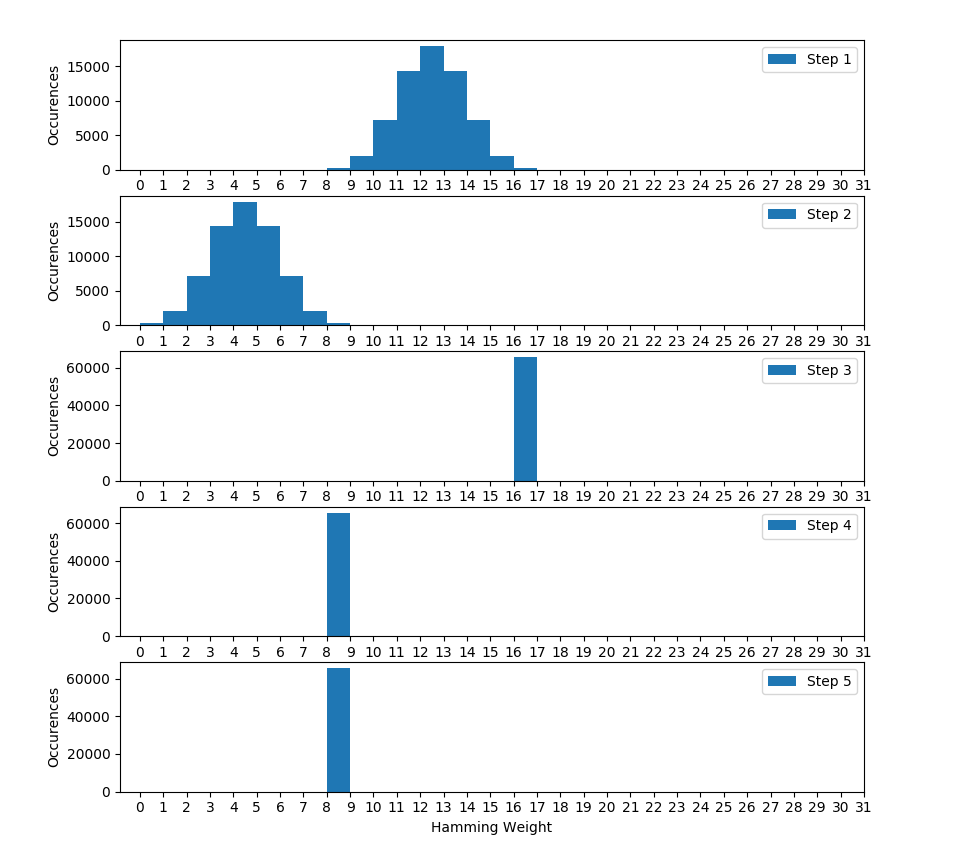
\includegraphics[width=\textwidth]{orr.png}
    \end{column}
    }
  \end{columns}
\end{frame}

\againframe<5>{overview}

\subsection{Compiler Pass}
\begin{frame}
  \frametitle{Applying the changes}
  Possibilities for automatic balancing:
  \begin{itemize}
  \item Transform source
  \item Transform during compilation
  \end{itemize}

  \vfill
  \onslide<2->{
  LLVM:
  \begin{figure}
  \centering
  \begin{tikzpicture}
    \node[draw, minimum width=1.3cm, minimum height=0.6cm] at (-2.5,1.5) (C) {C};
    \node[draw, minimum width=1.3cm, minimum height=0.6cm] at (-2.5,0.5) (C++) {C++};
    \node[draw, minimum width=1.3cm, minimum height=0.6cm] at (-2.5, -0.5) (Haskell) {Haskell};
    \node[draw, minimum width=1.3cm, minimum height=0.6cm] at (-2.5, -1.5) (otherl) {...};
    \node[draw] at (-0.75, 0) (irl) {IR};
    
    \node[draw, label=Optimizer Passes, minimum width=4cm, minimum height=1.3cm] at (2,0) (optimization) {};
    \node[draw, minimum size=0.5cm] at (0.6,0) {};
    \node[draw, minimum size=0.5cm] at (1.2,0) {};
    \node[draw, minimum size=0.5cm] at (1.8,0) {};
    \node[draw, minimum size=0.5cm] at (2.4,0) {};
    \node at (3.0, 0) {...};

    \node[draw] at (4.75, 0) (irr) {IR};
    \node[draw, minimum width=1.3cm, minimum height=0.6cm] at (6.5,1) (x86) {x86};
    \node[draw, minimum width=1.3cm, minimum height=0.6cm] at (6.5,0) (arm) {ARM};
    \node[draw, minimum width=1.3cm, minimum height=0.6cm] at (6.5,-1) (otherr) {...};

    \draw[->] (C) -- (irl);
    \draw[->] (C++) -- (irl);
    \draw[->] (Haskell) -- (irl);
    \draw[->] (otherl) -- (irl);

    \draw[->] (irl) -- (optimization);
    \draw[->] (optimization) -- (irr);

    \draw[->] (irr) -- (x86);
    \draw[->] (irr) -- (arm);
    \draw[->] (irr) -- (otherr);

    \onslide<3>{
    \node[draw, minimum height=0.6cm] (balance) at (3,-2) {Balance.cpp};
    \draw[->, uibkorange, line width=0.3mm, shorten <= 5pt] (balance) -- (3,-0.2);
    }
  \end{tikzpicture}
  \end{figure}
  }
\end{frame}

\begin{frame}[fragile]
  \frametitle{Optimizer Pass}

  \begin{columns}[T]
    \begin{column}{0.3\textwidth}
      Transforms:
      \begin{itemize}
      \item function arguments
      \item allocations
      \item stores
      \item \textcolor<2>{uibkorange}{loads} \quad \onslide<2>{\tikz[baseline=-0.5ex]{\draw[->, uibkorange, line width=0.3mm](0,0) -- (2,0);}}
      \item casts
      \item binary operators
      \item getElementPtr
      \item compares
      \item returns
      \item function calls
      \end{itemize}
    \end{column}
    \hfill
    \pause
    \vrule
    \hfill
    \begin{column}{0.6\textwidth}
      \begin{lstlisting}[language=C++,basicstyle=\small]
void balanceLoad(LoadInst *load,
    IRBuilder<> builder,
    vector<Instruction *> &to_remove,
    unordered_set<Value *> &balanced_values) {
  if (balanced_values
      .count(load->getPointerOperand())) {
    `\tikzmarkin{a}(3.3,-.15)(-0.1,.3)`auto *new_load = builder
        .CreateLoad(load->getPointerOperand());
    load->replaceAllUsesWith(new_load);
    balanced_values.insert(new_load);
    to_remove.push_back(load);`\tikzmarkend{a}`
    return;
  }
}
      \end{lstlisting}
    \end{column}
  \end{columns}
\end{frame}

\begin{frame}[fragile]
  \frametitle{Binary operators}
  \begin{columns}[T]
    \begin{column}{.48\textwidth}
      \begin{itemize}
      \item[] written as C functions
      \item[] linked into same module
      \item[] llvm operators changed to calls
      \end{itemize}
      \vfill
      \begin{block}{Tradeoff}
        \begin{itemize}
        \item[+] simplicity
        \item[+] modularity
        \item[+] small binaries
        \item[-] (currently) on inlining
        \item[-] overhead
        \end{itemize}
      \end{block}
    \end{column}
    \hfill
    \pause
    \begin{column}{.48\textwidth}
      \vspace{0.7cm}
      \begin{lstlisting}[language=C, basicstyle=\small]
uint32_t balanced_or(uint32_t lhs,
        uint32_t rhs) {
  uint32_t temp_or = lhs | rhs;
  uint32_t temp_and = lhs & rhs;
  uint32_t combined = (temp_and << 8)
          | temp_or;
  combined &= 0xff0000ff;
  return balanced_2_1(combined);
}
      \end{lstlisting}
    \end{column}
  \end{columns}
\end{frame}


\begin{frame}[fragile]
  \frametitle{Optimizer Pass cont.}
  \begin{columns}[T]
    \begin{column}{0.4\textwidth}
      \begin{lstlisting}[language=LLVM, basicstyle=\small]
%2 = alloca i8, align 1
store i8 %0, i8* %2, align 1
%3 = load i8, i8* %2, align 1
%4 = zext i8 %3 to i32
%5 = shl i32 %4, 1
%6 = load i8, i8* %2, align 1
%7 = zext i8 %6 to i32
%8 = ashr i32 %7, 7
%9 = and i32 %8, 1
%10 = mul nsw i32 %9, 27
%11 = xor i32 %5, %10
%12 = trunc i32 %11 to i8
ret i8 %12
      \end{lstlisting}
    \end{column}
    %% \hfill
    \vrule
    \hfill
    \begin{column}{0.48\textwidth}
      \begin{lstlisting}[language=LLVM, basicstyle=\small]
%2 = alloca i32
store i32 %0, i32* %2, align 1
%3 = load i32, i32* %2
%4 = call i32
  @balanced_shl(i32 %3, i32 0xfe0001)
%5 = load i32, i32* %2
%6 = call i32
  @balanced_ashr(i32 %5, i32 0xf80007)
%7 = call i32
  @balanced_and(i32 %6, i32 0xfe0001)
%8 = call i32
  @balanced_mul(i32 %7, i32 0xe4001b)
%9 = call i32
  @balanced_xor(i32 %4, i32 %8)
ret i32 %9
      \end{lstlisting}
    \end{column}
  \end{columns}
\end{frame}

\subsection{Results}

\againframe<6>{overview}

\subsection{Evaluation}
\begin{frame}
  \frametitle{Evaluation}

  How to generate ``virtual'' power traces?
  
  \begin{block}{Qemu alone}
    \begin{itemize}
    \item[+] fast
    \item[-] wrong resolution
    \end{itemize}
  \end{block}

  \begin{alertblock}{Qemu + gdb}
    \begin{itemize}
    \item[+] correct resolution
    \item[+] includes program location information
    \item[-] \textbf{very} slow
    \end{itemize}
    Execute instruction by instruction, dump registers every time
  \end{alertblock}
\end{frame}

\begin{frame}[label=results]
  \frametitle{Results}
  \center
  \vfill
  \begin{tabular}{|l|l|l|}
    \hline
    & \multicolumn{2}{c|}{AES} \\
    \cline{2-3}
    & unbalanced & balanced \\
    \cline{2-3}
    No. of instructions & 22 876 & 339 168 \\
    Relative increase & 1 & 14.888 \\
    Balanced operations & 20 571 & 334 521 \\
    Unbalanced operations & 2211 & 4647 \\
    Balancedness      & 0.903 & 0.986 \\
    Code size         & 76 KB & 78 KB \\
    \hline
  \end{tabular}
  \vfill
\end{frame}

\begin{frame}
  \begin{figure}
    \centering
    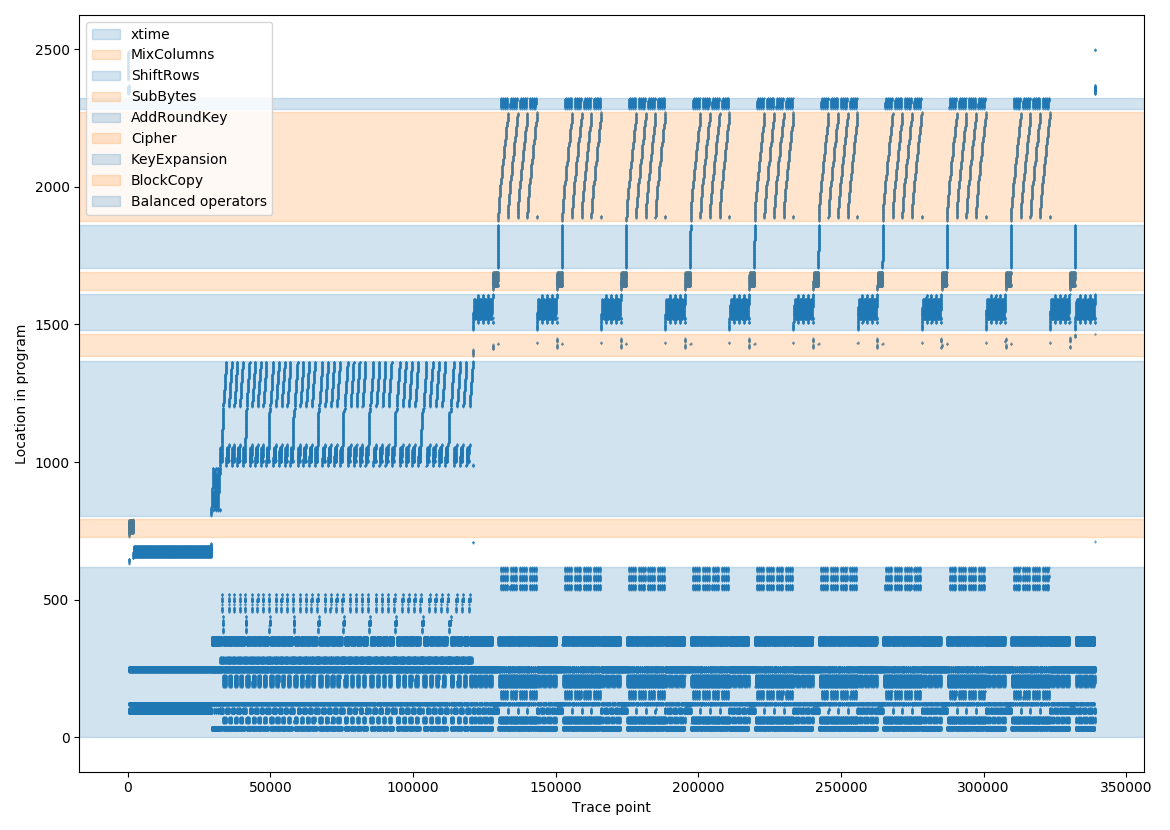
\includegraphics[height=\textheight]{aes-parts.png}
  \end{figure}
\end{frame}

\begin{frame}
  \begin{figure}
    \centering
    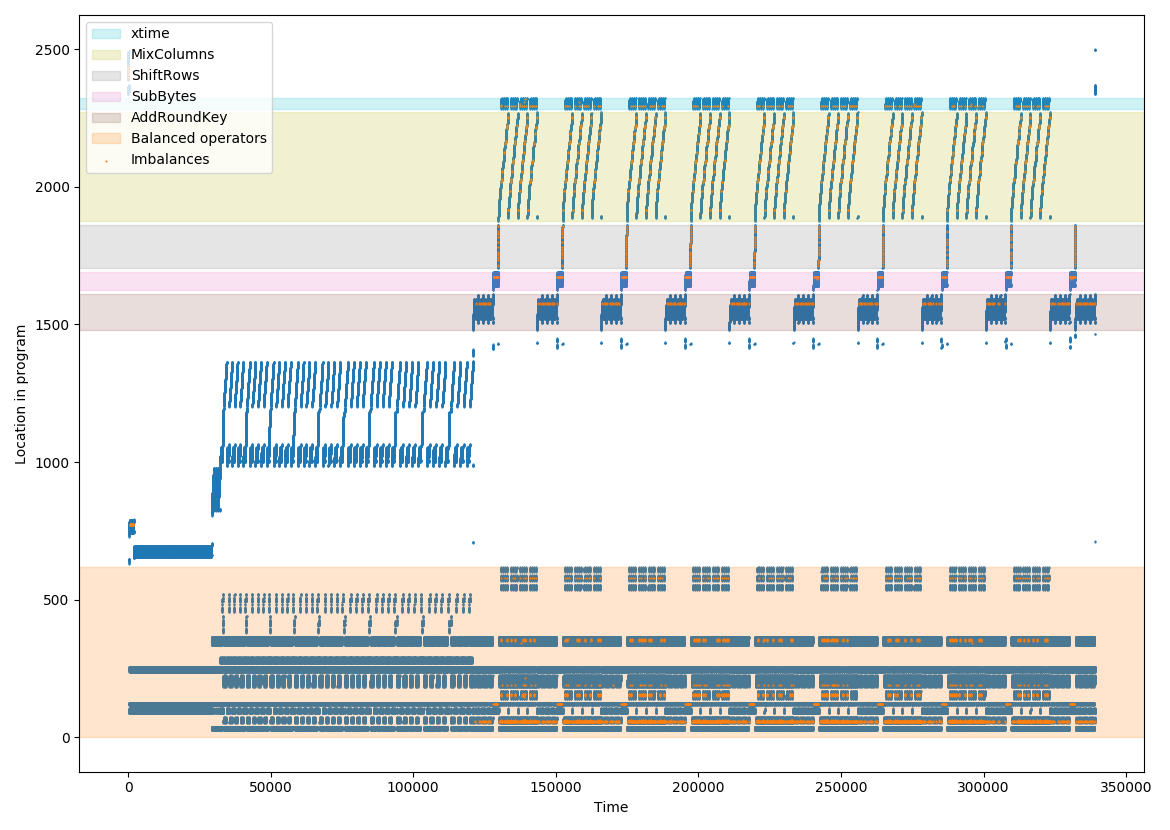
\includegraphics[height=\textheight]{imbalances-0.png}
  \end{figure}
\end{frame}

\begin{frame}
  \begin{figure}
    \centering
    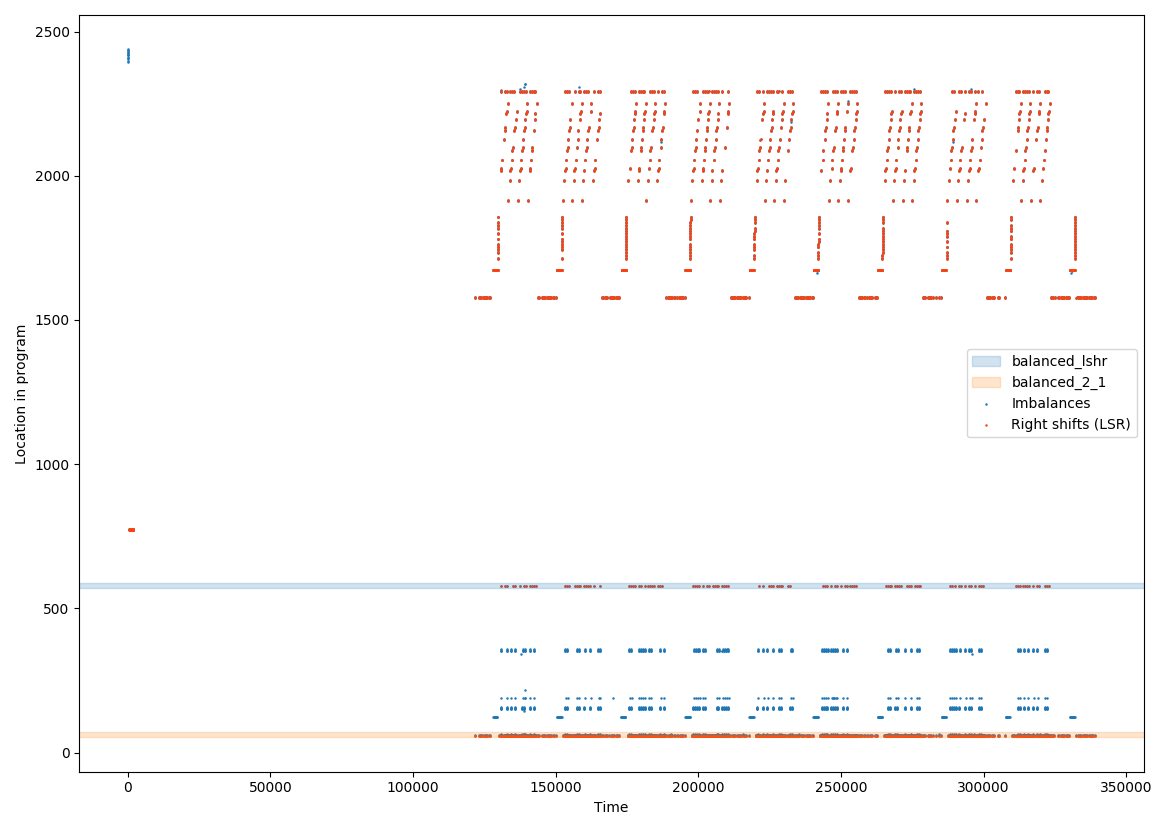
\includegraphics[height=\textheight]{imbalances-1.png}
  \end{figure}

\end{frame}
\begin{frame}
  \begin{figure}
    \centering
    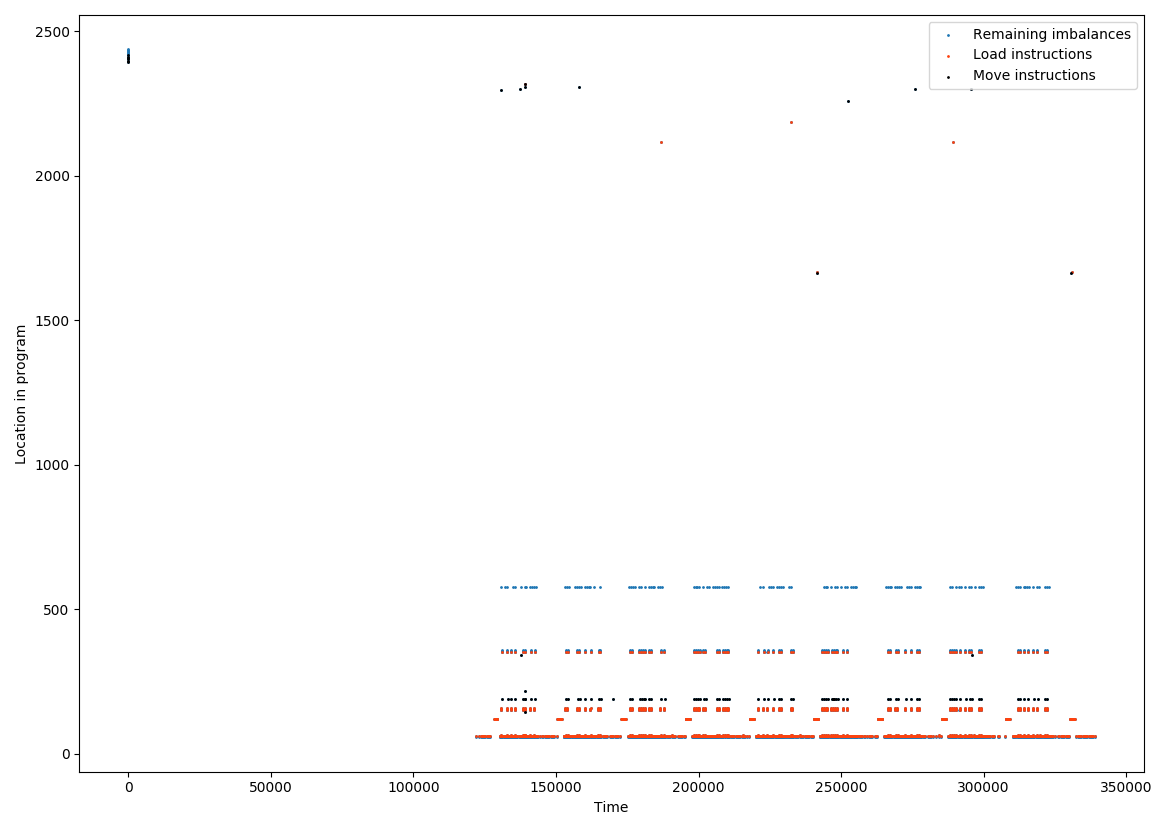
\includegraphics[height=\textheight]{imbalances-2.png}
  \end{figure}

\end{frame}
\begin{frame}
  \begin{figure}
    \centering
    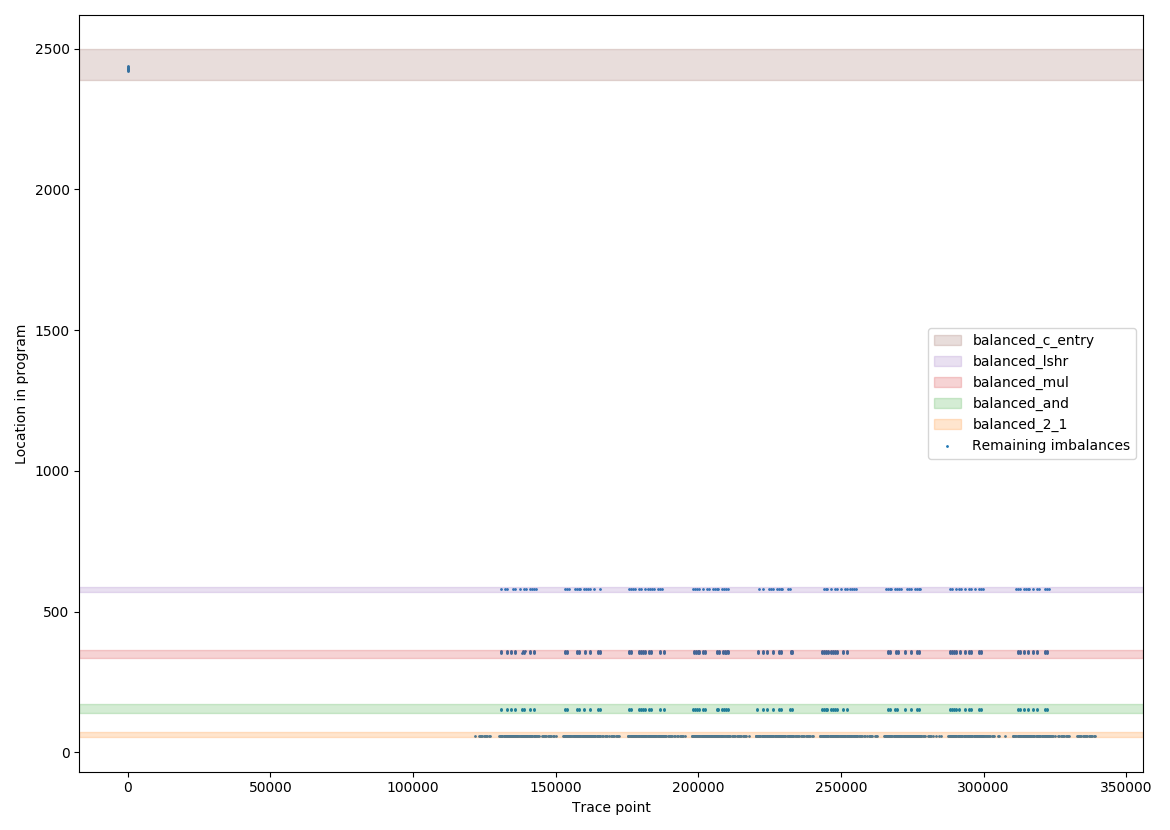
\includegraphics[height=\textheight]{imbalances-3.png}
  \end{figure}
\end{frame}

\againframe{results}

\begin{frame}
  \frametitle{Filtered Results}
  \vfill
  \begin{center}
  \begin{tabular}{|l|l|l|}
    \hline
    & \multicolumn{2}{c|}{AES} \\
    \cline{2-3}
    & unbalanced & balanced \\
    \cline{2-3}
    No. of instructions & 22 876 & 339 168 \\
    Relative increase & 1 & 14.888 \\
    Balanced operations & 20 571 & \textcolor{uibkorange}{\textbf{337 852}} \\
    Unbalanced operations & 2211 & \textcolor{uibkorange}{\textbf{1316}} \\
    Balancedness      & 0.903 & \textcolor{uibkorange}{\textbf{0.996}} \\
    Code size         & 76 KB & 78 KB \\
    \hline
  \end{tabular}
  \end{center}
  \vspace{1ex}
  Note: no filtering applied to unbalanced variant
  \vfill
\end{frame}

\againframe<7>{overview}

\subsection{Future Work}
\begin{frame}
  \frametitle{Future work}
  Same idea with different methods:
  \begin{itemize}
  \item Test on actual hardware
  \item Balance globals
  \item Improve operators
  \item Mark balancing targets
  \item Move balancing to type system
  \end{itemize}
  \vspace{0.5cm}
  Different ideas with same method:
  \begin{itemize}
  \item Other power analysis defenses
  \item Control flow randomization
  \item Move more security tools to LLVM
  \end{itemize}
\end{frame}

\subsection{Conclusion}
\begin{frame}
  \frametitle{Conclusion}
  \begin{itemize}
  \item Increased robustness without program modifications
  \item Requires more powerful, but standard hardware
  \item Security and performance likely mutually exclusive
  \item Backend cannot entirely be ignored
  \item Qemu is not a processor emulator
  \end{itemize}
  \vfill
  \begin{block}{LLVM IR}
    LLVM's intermediate representation offers many avenues for future work,\\
    not only for optimizition, but also for security.
  \end{block}
\end{frame}

\end{document}
